% SENSORS_MINIMUM.tex — companion to SENSORS.md.
% Hand-maintained prose. Every number marked "computed" comes from
% model/electrode_fim.jl; every number marked "served" is read from api/stream/.
% Build:  pdflatex SENSORS_MINIMUM.tex   (twice, for the page count)

\documentclass[10pt,a4paper]{article}
\usepackage[a4paper,top=1.5cm,bottom=1.5cm,left=1.7cm,right=1.7cm]{geometry}
\usepackage[T1]{fontenc}
\usepackage[utf8]{inputenc}
\usepackage{textcomp}
\usepackage{lmodern}
\usepackage{charter}
\usepackage[scaled=0.88]{helvet}
\usepackage{amsmath,amssymb}
\usepackage{xcolor}
\usepackage{colortbl}
\usepackage{tikz}
\usepackage{tcolorbox}
\usepackage{booktabs}
\usepackage{array}
\usepackage{tabularx}
\usepackage{enumitem}
\usepackage{microtype}
\usepackage{listings}
\usepackage{fancyhdr}
\usetikzlibrary{calc,decorations.pathmorphing,arrows.meta,shapes.geometric,positioning}
\tcbuselibrary{skins,breakable}

%========================================================= palette
\definecolor{ink}{HTML}{16212B}
\definecolor{mid}{HTML}{45555F}
\definecolor{faint}{HTML}{7D8B95}
\definecolor{rulec}{HTML}{D3DBE1}
\definecolor{paper}{HTML}{F5F8F9}

\definecolor{elec}{HTML}{0D6B73}   % the electrodes / impedance
\definecolor{cuff}{HTML}{2A6099}   % the blood-pressure cuff
\definecolor{ecg}{HTML}{6D4AA0}    % the ECG leads
\definecolor{bolt}{HTML}{B1541F}   % the thing we are refusing to place
\definecolor{warn}{HTML}{C0821A}
\definecolor{crit}{HTML}{BE3B3B}
\definecolor{ok}{HTML}{2E8B57}
\definecolor{grey}{HTML}{94A3B8}
\definecolor{skin}{HTML}{E8DED4}
\definecolor{vein}{HTML}{3E6EA8}

\setlength{\parindent}{0pt}
\setlength{\parskip}{4pt}
\pagestyle{fancy}\fancyhf{}
\renewcommand{\headrulewidth}{0pt}
\fancyfoot[L]{\sffamily\scriptsize\color{faint}SENSORS\_MINIMUM \;\textperiodcentered\;
  companion to SENSORS.md \;\textperiodcentered\; \textbf{design, not result}}
\fancyfoot[R]{\sffamily\scriptsize\color{faint}\thepage}

%========================================================= furniture
\newcounter{seccnt}
\newcommand{\Sec}[2][elec]{\par\addvspace{11pt}\noindent
  \refstepcounter{seccnt}%
  \begin{tikzpicture}[baseline=(t.base)]
    \node[fill=#1,text=white,rounded corners=1.5pt,inner xsep=4pt,inner ysep=2pt,
          font=\sffamily\bfseries\scriptsize] (n) {\theseccnt};
    \node[right=4.5pt of n,anchor=west,font=\sffamily\bfseries\normalsize,text=ink,
          inner sep=0] (t) {\MakeUppercase{#2}};
  \end{tikzpicture}\par
  \vspace{2.5pt}{\color{rulec}\hrule height .7pt}\vspace{5pt}}

\newcommand{\Sub}[1]{\par\addvspace{5pt}%
  {\sffamily\bfseries\footnotesize\color{mid}\MakeUppercase{#1}}\par\vspace{1pt}}

\newtcolorbox{cbox}[2][elec]{enhanced,breakable,
  colback=#1!6!white,colframe=#1,boxrule=0pt,leftrule=3pt,
  arc=1pt,outer arc=1pt,left=9pt,right=9pt,top=6.5pt,bottom=6.5pt,
  before upper={\sffamily\bfseries\footnotesize\color{#1}\MakeUppercase{#2}%
                \par\vspace{2.5pt}\normalfont\small\color{ink}}}

% a status chip
\newcommand{\chip}[2]{\tikz[baseline=-.65ex]{\node[fill=#1,text=white,rounded corners=1.2pt,
  inner xsep=3.2pt,inner ysep=1.4pt,font=\sffamily\bfseries\fontsize{6.4}{6.4}\selectfont]
  {\MakeUppercase{#2}};}}
\newcommand{\yes}{{\color{ok}$\bullet$}}
\newcommand{\no}{{\color{grey}$\circ$}}

\lstset{
  basicstyle=\ttfamily\scriptsize\color{ink},
  backgroundcolor=\color{paper},
  frame=leftline, framerule=2.2pt, rulecolor=\color{elec!45},
  keywordstyle=\color{elec}\bfseries,
  commentstyle=\color{faint}\itshape,
  stringstyle=\color{cuff},
  showstringspaces=false, breaklines=true, extendedchars=true, columns=fullflexible,
  xleftmargin=9pt, framexleftmargin=9pt, framexrightmargin=3pt,
  framextopmargin=3pt, framexbottommargin=3pt,
  aboveskip=7pt, belowskip=5pt,
  morekeywords={function,end,return,for,in,if,else,elseif,const,using,include,do,let,struct},
  literate={θ}{{\ensuremath{\theta}}}1 {σ}{{\ensuremath{\sigma}}}1 {Δ}{{\ensuremath{\Delta}}}1
           {Ω}{{\ensuremath{\Omega}}}1 {·}{{\ensuremath{\cdot}}}1 {—}{{---}}1
           {→}{{\ensuremath{\rightarrow}}}1 {≥}{{\ensuremath{\ge}}}1 {≤}{{\ensuremath{\le}}}1
}

\begin{document}

%========================================================= hero
\begin{tikzpicture}[remember picture,overlay]
  \fill[ink] ($(current page.north west)+(0,0)$) rectangle
             ($(current page.north east)+(0,-4.15cm)$);
  \fill[elec] ($(current page.north west)+(0,-4.15cm)$) rectangle
              ($(current page.north east)+(0,-4.28cm)$);
\end{tikzpicture}
\vspace*{-0.35cm}
{\color{white}\sffamily
  {\fontsize{8}{8}\selectfont\color{elec!35!white}\textbf{COMPANION TO SENSORS.MD \;\textperiodcentered\;
   TIER 0}}\\[7pt]
  {\fontsize{27}{29}\selectfont\bfseries SENSORS\_MINIMUM}\\[5pt]
  {\fontsize{12.5}{15}\selectfont A jugular compression with a blood-pressure cuff\\
   and seven electrodes --- and no burr hole.}\\[9pt]
  {\fontsize{8.2}{8.2}\selectfont\color{white!62!ink}%
  \tikz[baseline=-.6ex]\filldraw[cuff] (0,0) circle (1.5pt);\, 1 CUFF \quad
  \tikz[baseline=-.6ex]\filldraw[elec] (0,0) circle (1.5pt);\, 4 NECK ELECTRODES \quad
  \tikz[baseline=-.6ex]\filldraw[ecg] (0,0) circle (1.5pt);\, 3 ECG ELECTRODES \quad
  \tikz[baseline=-.6ex]\filldraw[bolt] (0,0) circle (1.5pt);\, 0 INTRACRANIAL DEVICES}
}
\vspace{1.05cm}

\begin{cbox}[warn]{Design, not result}
Nothing here was measured. \textbf{There is no impedance channel in this dataset}, so no
estimator in this document has ever been run against a real electrode signal.

Everything marked \textbf{computed} comes from \texttt{model/electrode\_fim.jl}, a Fisher
analysis of the model's \emph{own} synthetic observable at the operating point the API
publishes today --- it says what the model thinks an electrode would identify, which is a
statement about the model. Everything marked \textbf{served} is read out of
\texttt{api/stream/}. Everything else is engineering argument.

Read this as the specification for an experiment, not as its outcome.
\end{cbox}

%========================================================= 1
\Sec{The question SENSORS.md stops at}

\texttt{SENSORS.md} works out that the estimator behind \texttt{api/stream/} consumes one
invasive signal, one scalar and a stopwatch --- and then hits a wall: intracranial pressure
cannot be measured from outside the skull, so Tier~1 needs a burr hole and the
neurosurgical capability to make one.

This document refuses the burr hole and keeps the manoeuvre. \textbf{What can a
blood-pressure cuff and a handful of adhesive electrodes estimate about a jugular
compression?}

\begin{cbox}[elec]{The answer, in one sentence}
The cuff and the electrodes \textbf{cannot replace the bolt} --- four of the six streamed
parameters go dark and a fifth barely moves --- but they measure, better than the bolt
does, the one parameter the \textsc{rulebook} says the bolt-based fit is
\textbf{lying about}.
\end{cbox}

It is not a diagnostic tier. It is an \textbf{audit} tier: seven electrodes and a cuff,
pointed not at the patient but at the model.

%========================================================= 2
\Sec{The kit}

\vspace{-2pt}
\begin{center}
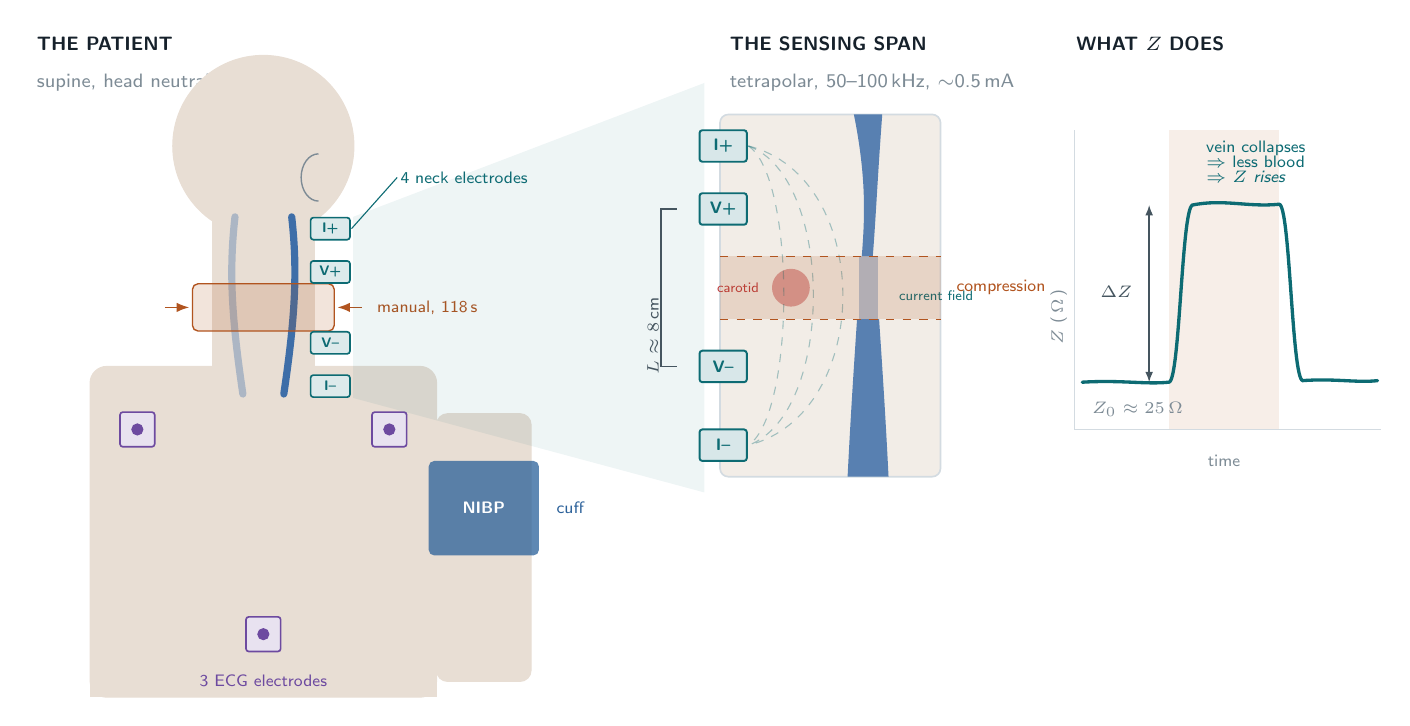
\begin{tikzpicture}[x=1mm,y=1mm,font=\sffamily]

%------------------------------------------------ left: the patient, schematic
\node[font=\sffamily\bfseries\scriptsize,text=ink,anchor=west] at (0,101) {THE PATIENT};
\node[font=\sffamily\scriptsize,text=faint,anchor=west] at (0,96)
  {supine, head neutral and \emph{fixed}};

% torso + shoulders
\fill[skin] (8,18) rectangle (52,58);
\draw[rounded corners=6pt,skin,fill=skin] (8,18) rectangle (52,60);
% arm
\draw[rounded corners=4pt,skin,fill=skin] (52,20) rectangle (64,54);
% neck
\fill[skin] (23.5,56) rectangle (36.5,76);
% head
\filldraw[skin,draw=skin] (30,88) circle (11.5);
\fill[skin] (23.5,74) rectangle (36.5,80);
% ear
\draw[faint,line width=.5pt] (37,87) arc (90:270:2.2 and 3);

% the internal jugular, running the neck
\draw[vein,line width=2.6pt,line cap=round] (33.6,79) .. controls (34.4,72) and (34.0,66) .. (32.6,56.5);
\draw[vein,line width=2.6pt,line cap=round,opacity=.35] (26.4,79) .. controls (25.6,72) and (26.0,66) .. (27.4,56.5);

% compression band
\fill[bolt,opacity=.16,rounded corners=2pt] (21,64.5) rectangle (39,70.5);
\draw[bolt,line width=.5pt,rounded corners=2pt] (21,64.5) rectangle (39,70.5);
\draw[bolt,-{Latex[length=1.6mm]},line width=.6pt] (17.5,67.5) -- (20.6,67.5);
\draw[bolt,-{Latex[length=1.6mm]},line width=.6pt] (42.5,67.5) -- (39.4,67.5);
\node[font=\sffamily\fontsize{6}{6}\selectfont,text=bolt,anchor=west] at (43.2,67.5)
  {manual, 118\,s};

% neck electrodes (right side of the neck)
\foreach \y/\lab in {77.5/I+,72.0/V+,63.0/V--,57.5/I--} {
  \draw[elec,fill=elec!14,rounded corners=1pt,line width=.6pt] (36.0,\y-1.4) rectangle (41.0,\y+1.4);
  \node[font=\sffamily\bfseries\fontsize{5.4}{5.4}\selectfont,text=elec] at (38.5,\y) {\lab};
}
\draw[elec,line width=.4pt] (41.2,77.5) -- (47,84) node[right,font=\sffamily\fontsize{6}{6}\selectfont,text=elec,inner sep=1pt] {4 neck electrodes};

% ECG
\foreach \x/\y in {14/52, 46/52, 30/26} {
  \filldraw[ecg,fill=ecg!16,rounded corners=1pt,line width=.6pt] (\x-2.2,\y-2.2) rectangle (\x+2.2,\y+2.2);
  \filldraw[ecg] (\x,\y) circle (.7);
}
\node[font=\sffamily\fontsize{6}{6}\selectfont,text=ecg,anchor=north] at (30,22) {3 ECG electrodes};

% cuff
\fill[cuff,opacity=.75,rounded corners=2pt] (51,36) rectangle (65,48);
\node[font=\sffamily\bfseries\fontsize{5.6}{5.6}\selectfont,text=white] at (58,42) {NIBP};
\node[font=\sffamily\fontsize{6}{6}\selectfont,text=cuff,anchor=west] at (66,42) {cuff};

%------------------------------------------------ zoom wedge
\fill[elec,opacity=.07] (41.4,79) -- (41.4,56) -- (86,44) -- (86,96) -- cycle;

%------------------------------------------------ right: the tetrapolar detail
\node[font=\sffamily\bfseries\scriptsize,text=ink,anchor=west] at (88,101) {THE SENSING SPAN};
\node[font=\sffamily\scriptsize,text=faint,anchor=west] at (88,96)
  {tetrapolar, 50--100\,kHz, ${\sim}$0.5\,mA};

% neck segment
\draw[rounded corners=3pt,fill=skin!55,draw=rulec,line width=.6pt] (88,46) rectangle (116,92);
% vein through it, tapered at the compression
\fill[vein,opacity=.85]
  (105,92) .. controls (106.6,84) and (106.4,79) .. (106.0,74)
  -- (107.4,74) .. controls (107.8,79) and (108.0,84) .. (108.6,92) -- cycle;
\fill[vein,opacity=.85]
  (105.4,66) .. controls (105.0,60) and (104.6,54) .. (104.2,46)
  -- (109.4,46) .. controls (109.0,54) and (108.6,60) .. (108.2,66) -- cycle;
\fill[vein,opacity=.35] (105.6,66) rectangle (108.0,74);
% carotid
\filldraw[crit,opacity=.45,draw=none] (97,70) circle (2.4);
\node[font=\sffamily\fontsize{5.2}{5.2}\selectfont,text=crit,anchor=east] at (94.2,70) {carotid};

% electrodes on the segment
\foreach \y/\lab in {88/I+,80/V+,60/V--,50/I--} {
  \draw[elec,fill=elec!16,rounded corners=1pt,line width=.7pt] (85.4,\y-2) rectangle (91.4,\y+2);
  \node[font=\sffamily\bfseries\fontsize{5.6}{5.6}\selectfont,text=elec] at (88.4,\y) {\lab};
}
% current field lines
\foreach \b in {6,11,16} {
  \draw[elec,opacity=.35,line width=.4pt,dashed]
    (91.6,88) .. controls (91.6+\b,84) and (91.6+\b,54) .. (91.6,50);
}
\node[font=\sffamily\fontsize{5.4}{5.4}\selectfont,text=elec,anchor=west] at (109.5,69)
  {current field};

% sense span brace
\draw[mid,line width=.5pt] (82.5,80) -- (80.5,80) -- (80.5,60) -- (82.5,60);
\node[font=\sffamily\fontsize{6}{6}\selectfont,text=mid,anchor=east,rotate=90] at (79.5,70)
  {$L\approx8$\,cm};

% compression on the detail
\fill[bolt,opacity=.16] (88,66) rectangle (116,74);
\draw[bolt,line width=.5pt,dashed] (88,66) -- (116,66);
\draw[bolt,line width=.5pt,dashed] (88,74) -- (116,74);
\node[font=\sffamily\fontsize{5.6}{5.6}\selectfont,text=bolt,anchor=west] at (116.8,70)
  {compression};

%------------------------------------------------ far right: what Z(t) does
\node[font=\sffamily\bfseries\scriptsize,text=ink,anchor=west] at (132,101) {WHAT $Z$ DOES};
\draw[rulec,line width=.6pt] (133,52) -- (133,90);
\draw[rulec,line width=.6pt] (133,52) -- (172,52);
\node[font=\sffamily\fontsize{6}{6}\selectfont,text=faint,anchor=east,rotate=90] at (131,71) {$Z$ (\,$\Omega$\,)};
\node[font=\sffamily\fontsize{6}{6}\selectfont,text=faint,anchor=north] at (152,50) {time};
% compression shading
\fill[bolt,opacity=.10] (145,52) rectangle (159,90);
% the trace: baseline, step up as the vein collapses, return
\draw[elec,line width=1.2pt,line cap=round]
  (134,58) .. controls (139,58.3) and (142,57.7) .. (145,58)
  .. controls (146.4,58) and (146.6,80) .. (148,80.5)
  .. controls (152,81.3) and (155,80.2) .. (159,80.6)
  .. controls (160.4,80.6) and (160.6,58.4) .. (162,58.2)
  .. controls (166,58.5) and (169,57.9) .. (171.5,58.2);
% delta Z arrow
\draw[mid,{Latex[length=1.3mm]}-{Latex[length=1.3mm]},line width=.5pt] (142.5,58) -- (142.5,80.5);
\node[font=\sffamily\fontsize{6}{6}\selectfont,text=mid,anchor=east] at (141.6,69.5) {$\Delta Z$};
\node[font=\sffamily\fontsize{5.6}{5.6}\selectfont,text=faint,anchor=west] at (134,54.6) {$Z_0\approx25\,\Omega$};
\node[font=\sffamily\fontsize{5.6}{5.6}\selectfont,text=elec,anchor=west,align=left] at (148.5,86)
  {vein collapses\\$\Rightarrow$ less blood\\$\Rightarrow$ $Z$ \emph{rises}};

\end{tikzpicture}
\end{center}
\vspace{-4pt}
{\footnotesize\color{faint}Schematic. Electrode positions indicate the anatomical region,
not a placement protocol. The sense span must straddle \textbf{the compressed segment} ---
see rule~E3.\par}

\vspace{4pt}
{\footnotesize
\begin{tabularx}{\linewidth}{@{}p{3.6cm} p{4.3cm} X@{}}
\toprule
\textbf{\sffamily Item} & \textbf{\sffamily What it is} & \textbf{\sffamily What it feeds in this repository}\\
\midrule
\chip{cuff}{cuff} \,Blood pressure & Any NIBP monitor; a manual sphygmomanometer serves &
  One scalar, \texttt{abp\_base}, the anchor for arterial resistance:
  \texttt{Ra0 = (abp\_base - 25.0)/12.5} (\texttt{model/ude\_cv.jl:128}). Tier~1 already
  needed only this number.\\[3pt]
\chip{elec}{neck} \,4 impedance electrodes & Tetrapolar array, outer pair injects, inner
  pair senses & \textbf{The new observable.} Neck venous volume, up to an unknown gain ---
  the model's state \texttt{u[11]}.\\[3pt]
\chip{ecg}{ecg} \,3 ECG electrodes & Any 3-lead cable & Beat gating, so the impedance pulse
  can be ensemble-averaged. Replaces the ABP waveform's role in Tier~2.\\[3pt]
\chip{bolt}{none} \,Stopwatch & --- & \texttt{t\_on} / \texttt{t\_off}. Unchanged from
  \texttt{SENSORS.md}.\\
\bottomrule
\end{tabularx}\par}

%========================================================= 3
\Sec{Why the model already contains what the electrodes see}

The pleasant surprise is that no new physics is required. The compact ODE carries thirteen
states, and the eleventh is the jugular cross-section:

\begin{lstlisting}
u = (V_a, C_a, q_avg, Pic, Pv, V_v, Psas, P_vv, P_px, P_sys, A, P_res, P_buf)
                                                            ^^^ u[11]
A_alg = P.A0 * tube_area((j - Pxt) / P.ktube)   # the tube law
dA    = (A_alg - A) / P.tauA                    # relaxes with tau_A = 20 ms
\end{lstlisting}

A tetrapolar neck measurement is a volume measurement. Blood is the most conductive tissue
in the neck, so filling the vein lowers $Z$ and collapsing it raises $Z$; Nyboer's relation
converts one to the other, $\Delta V = \rho\,(L/Z_0)^2\,\Delta Z$. The model's neck venous
volume is simply
\[
V_\mathrm{neck} \;=\; A \cdot \texttt{ltube} \cdot \texttt{Ntube}
\;=\; A \times 20\,\mathrm{cm} \times 2\ \text{veins},
\]
which \textbf{is} the electrode observable, up to a gain. So the question "what would
electrodes identify?" can be asked of the existing model directly --- and that is what
\texttt{model/electrode\_fim.jl} does.

\begin{cbox}[ok]{Is the signal even there? \normalfont\upshape (computed)}
At patient 081's published operating point the model swings the neck venous volume by
\textbf{158.9\,mL} across the manoeuvre. Through Nyboer with $\rho=150\,\Omega\,$cm,
$Z_0=25\,\Omega$ and an $L=8$\,cm sense span, that is
\[
\Delta Z \;\approx\; \mathbf{4.1\,\Omega}\ \text{on a }25\,\Omega\ \text{baseline}.
\]
Impedance cardiography routinely resolves $0.1\,\Omega$. Even if the real resting vein is
a third of the model's inflated one --- see \S6, it almost certainly is --- the swing is
still ${\sim}1.2\,\Omega$, an order of magnitude above a commodity noise floor.
\textbf{Signal availability is not the constraint here.} Identifiability is.
\end{cbox}

%========================================================= 4
\Sec{The gain problem, and why it is only half fatal}

An impedance electrode returns ohms, not millilitres. The conversion depends on neck
geometry, electrode spacing, haematocrit and body composition --- unknown per patient, and
not stable enough between patients to hard-code. Two honest responses, and the design uses
both:

\begin{cbox}[elec]{(a) Profile the gain out, do not assume it}
The observable scales linearly with the gain $g$, so $\partial\,\text{obs}/\partial\log g
= \text{obs}$. Append that as a seventh column of the sensitivity matrix, invert the
$7\times7$ Fisher matrix and read the six parameter variances off its diagonal. The cost of
not knowing $g$ then appears \emph{in the numbers} instead of being wished away. The
\textbf{electrode} column of the table in \S5 is computed this way; \textbf{elec+calib} is
the same calculation with that column removed --- what a perfectly calibrated electrode
would buy.
\end{cbox}

\begin{cbox}[elec]{(b) Use a statistic the gain cannot touch}
The \textbf{ratio} $A_\mathrm{plateau}/A_\mathrm{rest}$ is gain-free: $g$ cancels exactly.
It needs no calibration, no $\rho$, no assumed $L$ --- only a stable $Z_0$ (rule~E4). It is
also, by luck, the quantity that decides the \textsc{rulebook}'s signature failure.
\end{cbox}

%========================================================= 5
\Sec{What is identifiable --- computed}

\texttt{model/electrode\_fim.jl} builds the same Fisher matrix
\texttt{stream\_refit.jl:sigmas()} builds, with the same log-parameter step
($\delta=0.05$) and the same measurement noise on ICP ($\sigma=0.35$\,mmHg), but against
three observables. Impedance noise is set at 2\% of the manoeuvre's own excursion, so the
electrode gets a generous fixed 50:1 SNR.

\vspace{2pt}
{\footnotesize
\setlength{\tabcolsep}{5pt}
\renewcommand{\arraystretch}{1.25}
\begin{tabularx}{\linewidth}{@{}l X r r r r@{}}
\toprule
\textbf{\sffamily Fitted} & \textbf{\sffamily Streamed as} &
\textbf{\sffamily ICP only} & \textbf{\sffamily electrode} &
\textbf{\sffamily elec+calib} & \textbf{\sffamily both}\\
& & \scriptsize needs a bolt & \scriptsize gain unknown & \scriptsize gain known & \\
\midrule
\texttt{E}      & craniospinal compliance   & \cellcolor{ok!14}0.040 & \cellcolor{crit!13}78.0 & \cellcolor{crit!13}75.5 & \cellcolor{ok!14}0.040\\
\texttt{Psinus} & sagittal sinus pressure   & \cellcolor{ok!14}0.004 & \cellcolor{crit!13}63.0 & \cellcolor{crit!13}63.0 & \cellcolor{ok!14}0.004\\
\texttt{Ro\_tot}& CSF outflow resistance    & \cellcolor{ok!14}0.016 & \cellcolor{crit!13}91.1 & \cellcolor{crit!13}71.2 & \cellcolor{ok!14}0.016\\
\texttt{Rvvs}   & collateral outflow resist.& \cellcolor{ok!14}0.351 & \cellcolor{crit!13}63.4 & \cellcolor{crit!13}45.3 & \cellcolor{ok!14}0.268\\
\rowcolor{elec!7}
\texttt{k\_ijvs}& \textbf{jugular resting area} & \cellcolor{ok!14}\textbf{0.077} & \cellcolor{ok!14}\textbf{0.191} & \cellcolor{ok!30}\textbf{0.003} & \cellcolor{ok!14}\textbf{0.053}\\
\texttt{Ca}     & arterial compliance       & \cellcolor{ok!14}0.034 & \cellcolor{crit!13}7.18 & \cellcolor{crit!13}6.97 & \cellcolor{ok!14}0.034\\
\bottomrule
\end{tabularx}\par}
\vspace{2pt}
{\footnotesize\color{faint}Fractional (log-space) standard deviation. \textbf{Lower is
better}; the contract calls a parameter identifiable below \textbf{0.5}
(\texttt{IDENT\_MAX\_SIGMA}). Patient 081, final window, operating point read from
\texttt{api/stream/081\_batch} --- the expanding-window refit. \par}

\Sub{How to read it}

\begin{itemize}[leftmargin=13pt,itemsep=2.5pt,topsep=3pt]
\item \textbf{The electrodes identify exactly one parameter of six.} \texttt{k\_ijvs} at
$\sigma=0.191$; everything else lands between 7 and 91, which is two to three orders of
magnitude outside the threshold. No plausible improvement in electrode noise closes a gap
that size --- the conclusion is not sensitive to the 2\% SNR assumption.
\item \textbf{Uncalibrated, the electrode matches the bolt on that parameter} (0.191 vs
0.077, same order). \textbf{Calibrated, it beats the bolt by a factor of 26} (0.003 vs
0.077). The gain is worth roughly 60$\times$ on this coordinate and nothing at all on the
others.
\item \textbf{The collateral is not rescued.} This was the hypothesis going in --- that
electrodes would see the flow diverted into the vertebral plexus --- and the computation
says no ($\sigma=63$ alone, $0.351\rightarrow0.268$ jointly). The reason is mechanical: at
the fitted point the vein is already 97.8\% collapsed, so $R_j\propto A^{-2}$ is
effectively infinite and the neck volume is pinned at its floor no matter what the
collateral does. A sensor placed \emph{above} the compression would see the pooling
instead --- but the model has no state for it (rule~E3).
\item Re-run at the other published operating point for 081 (the filter stream, \S8) the
numbers move but the verdict does not: \texttt{k\_ijvs} $\sigma=0.161$, every other
parameter between 16 and 713.
\end{itemize}

%========================================================= 6
\Sec[crit]{What that one parameter is worth}

\texttt{jugular\_resting\_area} is not an incidental sixth of the output. It carries
\texttt{bound\_provenance: "qc"}, and its own metadata says why:

\begin{cbox}[bolt]{api/params/jugular\_resting\_area.json \normalfont\upshape (served)}
\emph{"STREAMED AS QUALITY CONTROL, NOT AS A DIAGNOSIS \dots\ the fit drives this to
5--12\,cm\textsuperscript{2} (about 205\,mL of jugular) which is roughly ten times
physiological, and that this artefact is what causes the model's ICP pulse-amplitude
failure. \textbf{A bedside ultrasound falsifies it in thirty seconds.} Read a value outside
the healthy band as evidence the \textsc{fit} is wrong, not that the patient is."}
\end{cbox}

Four neck electrodes are the version of that ultrasound which needs no operator, no probe
and no training --- and which runs continuously, through the manoeuvre, instead of once.
Here is what it would be falsifying. Every value below is real output, read from
\texttt{api/stream/}:

\vspace{2pt}
{\footnotesize
\setlength{\tabcolsep}{5.5pt}
\renewcommand{\arraystretch}{1.2}
\begin{tabularx}{\linewidth}{@{}l r r X l@{}}
\toprule
\textbf{\sffamily Patient} & \textbf{\sffamily Jugular resting area} &
\textbf{\sffamily vs.\ healthy ceiling} & \textbf{\sffamily Collateral resistance} &
\textbf{\sffamily Status}\\
& \scriptsize cm\textsuperscript{2}/vein, final window & \scriptsize $2.0$ &
\scriptsize mmHg/(mL/s) & \\
\midrule
081 \scriptsize(batch) & 4.50 & $2.2\times$ & 14.46 \chip{crit}{path} & \chip{crit}{R1 fires}\\
081 \scriptsize(filter) & 3.08 & $1.5\times$ & 2.01 \chip{grey}{unident} & \chip{warn}{masked}\\
083 & 2.55 & $1.3\times$ & 22.73 \chip{grey}{unident} & \chip{warn}{borderline}\\
137 & 4.47 & $2.2\times$ & 12.11 \chip{grey}{unident} & \chip{crit}{path.\ area}\\
150 & 8.32 & $4.2\times$ & 19.06 \chip{grey}{unident} & \chip{crit}{path.\ area}\\
\bottomrule
\end{tabularx}\par}
\vspace{3pt}

Every patient, every estimator: the resting jugular comes out above the physiological
ceiling, by between 1.3 and 4.2 times. \textsc{rulebook} R1 explains why --- the fit cannot
make the vein collapse hard enough to produce the measured ICP step, so it buys the step by
inflating the resting vein and blocking the collateral instead. \textbf{Neither number is a
statement about the patient.}

A neck electrode array settles this. It has two shots:

\begin{itemize}[leftmargin=13pt,itemsep=2.5pt,topsep=3pt]
\item \textbf{The absolute area}, which needs the calibration and is the decisive test:
162\,mL of resting jugular blood in a 20\,cm segment is either there or it is not.
\item \textbf{The gain-free collapse ratio}, which needs nothing. At 081's published point
the model collapses the vein to \textbf{2.2\% of resting} \emph{(computed)}. That is a
strong claim about a manoeuvre that is, after all, a pair of thumbs --- but it is a
\emph{weaker} test than the first, because near-complete collapse under firm manual
compression is not by itself implausible. Say so plainly: \textbf{the free test is the
weaker one.}
\end{itemize}

%========================================================= 7
\Sec{The implementation}

Six changes. Five are small, and the sixth is a decision rather than a change.

\Sub{1 --- the solver stores a third state}

\texttt{solve\_run} keeps \texttt{u[4]} and \texttt{u[5]} and discards the rest. The
electrode observable needs \texttt{u[11]}. This is the whole physics change:

\begin{lstlisting}
icp = Vector{T}(undef, nout); pv = Vector{T}(undef, nout)
ar  = Vector{T}(undef, nout)               # + jugular area
...
    k += 1; tout[k] = t; icp[k] = u[4]; pv[k] = u[5]; ar[k] = u[11]
\end{lstlisting}

\Sub{2 --- a second residual block, with its own noise scale}

\begin{lstlisting}
# neck venous volume the electrodes see, mL: both veins over the modelled segment
neckvol(a) = a .* P.ltube .* P.Ntube

function resid2(θ, t_end)
    t, icp, ar, ok = solve_obs(mkP(θ), REC); ok || return nothing
    ix = idxs(t, t_end)
    vcat((icp[ix] .- REC.icpm[ix2]) ./ σ_icp,        # empty in the electrode tier
         (neckvol(ar[ix]) .- Z_TO_ML .* REC.dz[ix2]) ./ σ_vol)
end
\end{lstlisting}

Blocks are pre-divided by their own $\sigma$, so the two observables are commensurable and
either can be dropped by supplying an empty block. \textbf{The electrode tier is the same
estimator with the first block empty.}

\Sub{3 --- the gain is profiled, not fitted}

Do not add $g$ to \texttt{PNAMES}. It is not a physiological quantity and it would collect
every modelling error that scales with amplitude. Append its column to the sensitivity
matrix inside \texttt{sigmas()} and drop it after the inversion:

\begin{lstlisting}
S = hcat(S, vol0)          # d obs / d log g == obs, for a linear gain
sigma = sqrt.(max.(diag(pinv((S'*S) ./ sigma_meas^2)), 0.0))[1:6]
\end{lstlisting}

\Sub{4 --- the streaming contract does not change}

This is the part worth pausing on. \texttt{model/stream\_contract.jl} fixes the six ids,
the derivations, the bounds and the exact bytes of a record --- and \emph{none of it needs
to move}. \texttt{emit\_record} already emits \texttt{"status": "unidentifiable"} with
\texttt{null} confidence bounds when $\sigma$ is unavailable, which is precisely what five
of the six parameters must now say. The electrode tier is not a new contract; it is the
existing contract, honestly filled in.

\Sub{5 --- the API surface does not change either}

Same routes, same record schema, same component translation. A client cannot distinguish an
electrode-tier stream from a bolt-tier one except by reading \texttt{identifiable} --- which
is the flag \texttt{CLAUDE.md} already instructs you to report \emph{instead of} the point
estimate. The discipline the API was built with is exactly what makes a degraded sensor tier
serveable without a schema change.

One caveat, and it is R9: an electrode estimator writing \texttt{api/stream/<patient>/} is a
\textbf{second writer}. It must take \texttt{take\_stream\_lock}, or write to its own
\texttt{\_SDIR} --- as \texttt{081\_batch} and \texttt{081\_filter} already do.

\Sub{6 --- one metadata decision, which is not ours to make silently}

If an electrode array actually measures the jugular area, then
\texttt{jugular\_resting\_area}'s \texttt{bound\_provenance} is no longer \texttt{"qc"}.
But it should \textbf{not} become \texttt{"clinical"} either: an impedance-derived area is
a device-dependent surrogate with a calibration in it, not a published human range. The
honest move is a fourth provenance value --- \texttt{"sensor"} --- and a matching sentence
in \texttt{CLAUDE.md}'s "what the numbers do and do not mean". Adding a provenance value is
an API contract change and belongs in \texttt{model/api\_spec.jl}, which rewrites
\texttt{api/index.json}.

%========================================================= 8
\Sec[warn]{An incidental finding, while we were in there}

\texttt{model/electrode\_fim.jl} reads its operating point back out of the published
stream. Doing that for 081 turned up something that has nothing to do with electrodes:

\begin{cbox}[warn]{api/stream/081 is byte-identical to api/stream/081\_filter}
All seven files, \texttt{cmp}-identical. \texttt{CLAUDE.md} describes \texttt{081\_filter}
as a different experiment, "not the canonical refit" --- which implies the canonical slot
holds the refit. It does not; it holds the filter run.

It matters because the filter run is the one \textsc{rulebook} R7 indicts by name:
\texttt{collateral\_outflow\_resistance} sits at \textbf{2.60588} for the first
\textbf{100+} windows with \texttt{n\_solves} frozen at 39 --- the Model 5 starting value,
never departed. And the two runs disagree about the finding: \texttt{081\_batch} reports the
collateral \textbf{pathological at 14.46 and identifiable}, which fires R1 cleanly alongside
a $4.50\,$cm\textsuperscript{2} jugular. The served \texttt{081} reports \textbf{2.01,
unidentifiable} --- R1 does not fire, and the artefact is invisible.

\textbf{Serving the frozen run hides the very failure the rulebook exists to expose.} Worth
a look independently of anything in this document.
\end{cbox}

%========================================================= 9
\Sec[crit]{What goes dark, and why it stays dark}

Two of the six do not merely become unidentifiable --- they become underivable, and the
distinction matters:

{\footnotesize
\setlength{\tabcolsep}{6pt}
\renewcommand{\arraystretch}{1.2}
\begin{tabularx}{\linewidth}{@{}l l X@{}}
\toprule
\textbf{\sffamily Parameter} & \textbf{\sffamily Loss} & \textbf{\sffamily Why}\\
\midrule
craniospinal compliance & \chip{crit}{underivable} &
  Its derivation is \texttt{1/(E * (icp\_base - 5.0))}. Even with a miraculous \texttt{E},
  the map to the clinical quantity divides by a \textbf{measured resting ICP} the electrode
  tier does not have. Two failures, not one.\\[2pt]
CSF outflow resistance & \chip{crit}{unidentifiable} &
  Lives in the slow ICP relaxation. There is no venous-volume signature of it
  ($\sigma=91$).\\[2pt]
sagittal sinus pressure & \chip{crit}{unidentifiable} &
  A pressure. $\sigma=63$.\\[2pt]
arterial compliance & \chip{warn}{degraded} &
  $\sigma=7.2$ from the mean-volume observable alone. The impedance \emph{pulse} --- ECG-gated,
  ensemble-averaged against the cuff pulse --- is a genuine volume-per-pressure ratio and is
  not in this calculation, which uses the 1\,Hz mean only. Treat the 7.2 as a floor on what
  is knowable, not a verdict on the pulse channel.\\[2pt]
collateral outflow resist. & \chip{crit}{unidentifiable} &
  \S5. Occluded veins tell you nothing about where the flow went.\\
\bottomrule
\end{tabularx}\par}

\vspace{3pt}
There is no clever recovery available here. Resting ICP is nearly blind to the venous
outflow path in one direction, and the venous volume is nearly blind to intracranial
mechanics in the other. \textbf{They are complementary observables, not substitutable
ones.} The right conclusion is not "electrodes instead of a bolt" but "electrodes
\emph{alongside} a bolt, where a bolt is justified --- and electrodes \emph{alone} to audit
the model, where it is not."

%========================================================= 10
\Sec{An electrode rulebook}

\texttt{RULEBOOK.md} lists the parameter combinations that indict the model. A sensor tier
needs its own, because these failures are not visible in any parameter value.

{\footnotesize
\setlength{\tabcolsep}{6pt}
\renewcommand{\arraystretch}{1.2}
\begin{tabularx}{\linewidth}{@{}l l X@{}}
\toprule
& \textbf{\sffamily Trigger} & \textbf{\sffamily What it means}\\
\midrule
\textbf{E1} & Head moves during the run &
  Jugular cross-section is posture-dependent --- that is in the metadata's own
  \texttt{bound\_source} string. A head turn changes $A$ without changing anything the
  model represents. \textbf{Fix the head, and record that you did.}\\[2pt]
\textbf{E2} & The plateau drifts &
  Respiratory venous modulation sits at 0.2--0.3\,Hz and is removed by the 1\,Hz mean, but a
  \emph{change in breathing pattern} across a 118\,s manoeuvre is not separable from a
  change in venous return. The bolt tier had this too; the electrode tier is worse, because
  the observable is a volume.\\[2pt]
\textbf{E3} & Sense span not over the compression &
  \textbf{The model has no spatial resolution and the electrode does.} \texttt{ltube} is one
  lumped 20\,cm collapsible tube under a uniform external pressure. A real compression is
  applied at one level: the vein collapses \emph{at} it and distends \emph{above} it. A span
  placed above the thumbs measures pooling --- a real and interesting signal --- which the
  model has no state for and will absorb into $A$ with the wrong sign.\\[2pt]
\textbf{E4} & $Z_0$ drifts &
  The gain-free ratio is only free if $Z_0$ is stable. Electrode--skin impedance moves with
  sweat, gel drying and movement; the ratio then moves with the vein standing still. Log
  $Z_0$ and reject the run if it drifts more than the manoeuvre's own $\Delta Z$.\\[2pt]
\textbf{E5} & The span is not purely venous &
  It contains carotid, muscle, skin and air. The gain is not merely unknown --- it is not a
  pure venous gain. Profiling $g$ absorbs a constant offset; it does not absorb an arterial
  component that moves with the cardiac cycle. This is what the ECG gating is for.\\[2pt]
\textbf{E6} & A second writer &
  R9, unchanged. An electrode estimator writing an existing patient directory truncates and
  interleaves silently.\\
\bottomrule
\end{tabularx}\par}

%========================================================= 11
\Sec{Verdict}

\begin{cbox}[elec]{Tier 0 --- one cuff, seven electrodes, no burr hole}
\textbf{Delivers:} one of six streamed parameters, \texttt{jugular\_resting\_area}, at
accuracy comparable to the bolt uncalibrated and $26\times$ better calibrated; a continuous
gain-free collapse ratio through the manoeuvre; a plausible route to the arterial-compliance
pulse channel via ECG-gated impedance. \textbf{No schema change, no route change, no new
physics.}

\textbf{Does not deliver:} intracranial pressure, or anything derived from it. Four
parameters unidentifiable, one of them underivable in principle.

\textbf{Is best understood as:} a continuous, operator-free version of the bedside
ultrasound that \texttt{api/params/jugular\_resting\_area.json} already names as the way to
falsify this model's signature artefact --- an instrument aimed at the fit rather than the
patient.
\end{cbox}

\vspace{4pt}
{\color{rulec}\hrule height .6pt}
\vspace{3pt}
{\scriptsize\color{faint}
\textbf{Provenance.} \textbf{Computed} --- the identifiability table, the volume swing, the
collapse ratio and the Nyboer estimate --- is output of
\texttt{model/electrode\_fim.jl}, run at 081's final published window
(\texttt{\_SRC=081\_batch} and \texttt{\_SRC=081}). It is a Fisher analysis of a
\emph{synthetic} observable derived from the model's own state \texttt{u[11]}; it reports
what the model believes an electrode would identify. \textbf{Served} --- the per-patient
table in \S6 and the byte-identity in \S8 --- is read from \texttt{api/stream/} and
\texttt{api/params/} as they stand on disk. \textbf{Everything else is engineering
argument.} No impedance signal exists in this dataset, no electrode estimator has been
written, and the electrode noise level, $\rho$, $Z_0$ and $L$ are literature-typical
assumptions, stated so they can be disagreed with.
\textbf{No healthy controls exist in this dataset} --- every bound is from literature.
The underlying model overestimates ICP pulse amplitude under compression by
${\sim}7\times$ from a diagnosed cause, which is the artefact this tier is aimed at.
Not clinical advice, and not a recommendation to place any monitor anywhere.}

\end{document}
